From HW~\ref{hw:ballbeam}.\ref{chap:transfer_function_models}, the transfer function for the inner loop of the ball \& beam is 
\begin{equation}\label{eq:hw_ballbeam_bode_in_tf}
P_{in}(s) = \frac{a}{s^2} = 
\frac{2.652}{s^2},
\end{equation}
where 
\[
a = \frac{\ell}{\frac{m_2\ell^2}{3}+m_1z_e^2}.
\]
In Bode canonical form we have
\[
P_{in}(j\omega) = \frac{2.652}{(j\omega)^2}
\]
Therefore
\begin{multline*} 
20\log_{10}\abs{P_{in}(j\omega)}=
	20\log_{10} 2.652 \\
	-40\log_{10}\abs{\omega}.
\end{multline*}
Therefore, the Bode plot for magnitude will be the graphical addition of a constant gain, and a line with slope of -40~dB/decade.
Similarly, the phase is given by
\[
\angle P_{in}(j\omega) = 
	\angle 2.652 
	- \angle (j\omega)
	- \angle (j\omega) = 0 - 90 - 90 = -180~\text{degrees}.
\]
The straight line approximation as well as the Bode plot generated by Matlab are shown in Figure~\ref{fig:hw_ballbeam_bode_in}.
\begin{figure}[H]
   \centering
   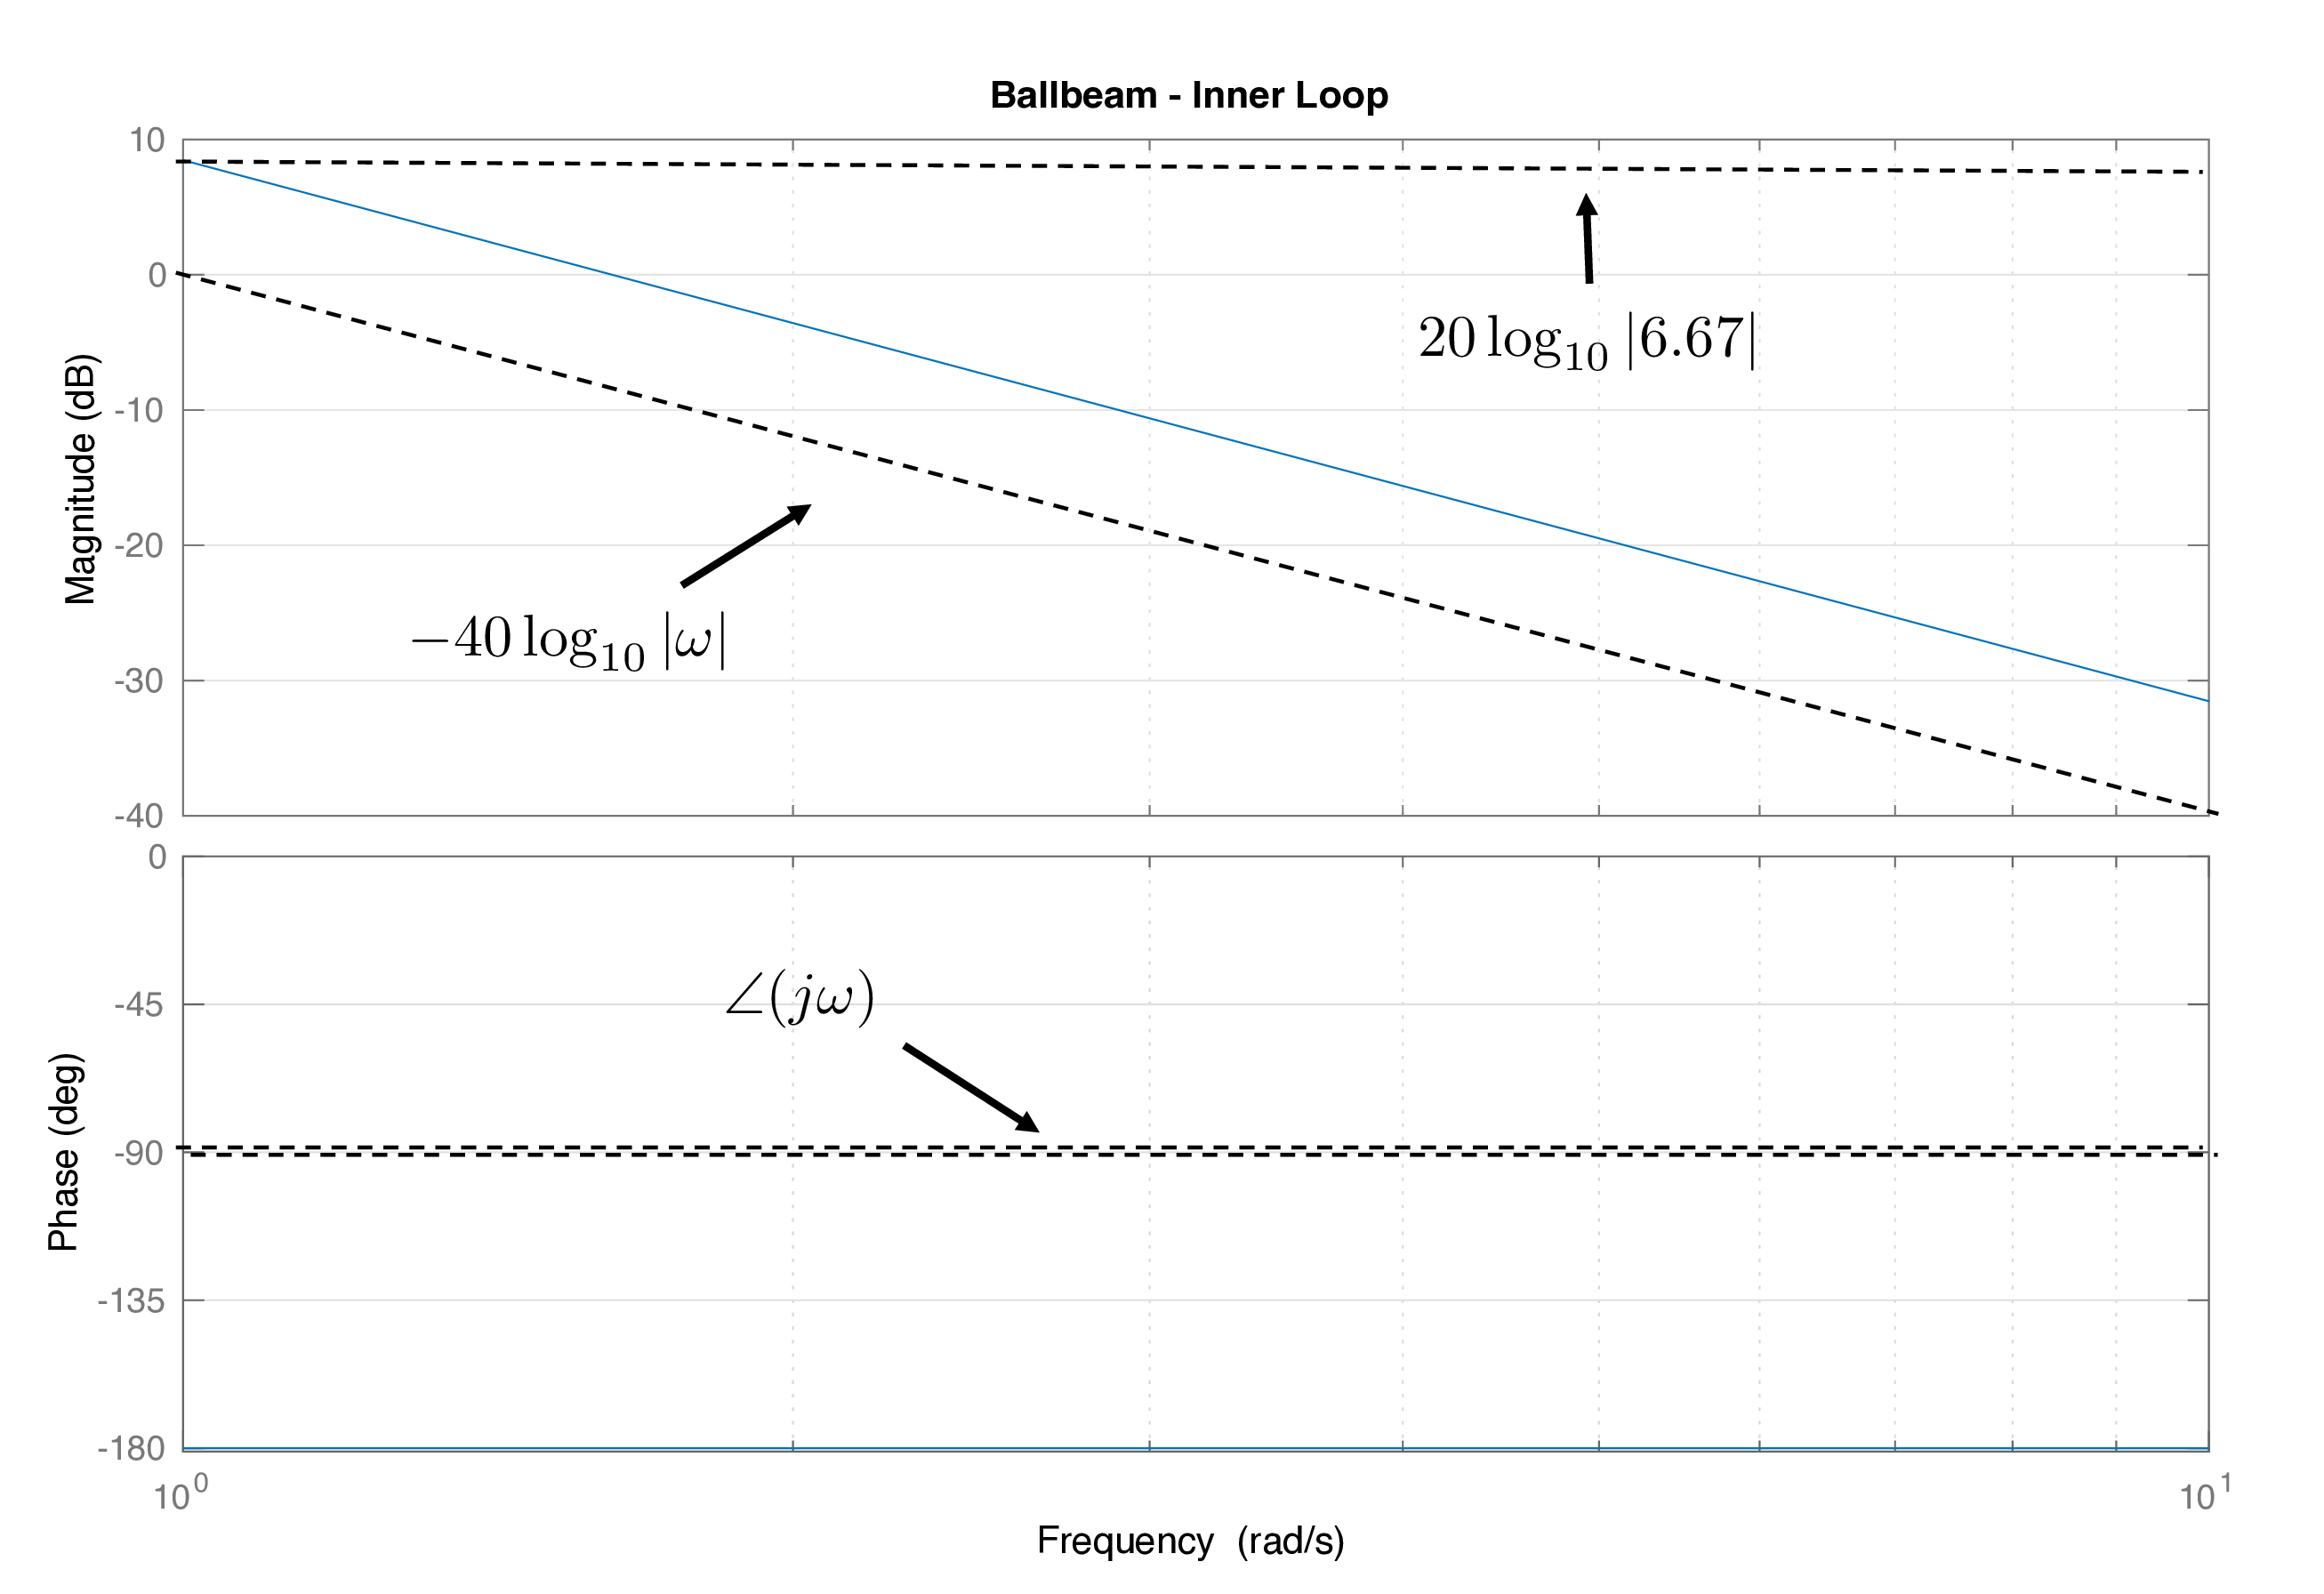
\includegraphics[width=0.9\textwidth]{6_design_studies/figures/hw_ballbeam_bode_in.pdf}
   \caption{Bode plot for the transfer function given in Equation~\eqref{eq:hw_ballbeam_bode_in_tf}.}
   \label{fig:hw_ballbeam_bode_in}
\end{figure}
%The Matlab command to generate the Bode plot is
%\begin{lstlisting}
%>> Pin = tf([2.652], [1, 0, 0]);
%>> figure(1), clf, bode(Pin), grid on
%\end{lstlisting}
The Python command to generate the Bode plot is
\begin{lstlisting}
	>> import matplotlib.pyplot as plt
	>> import control as cnt
	>> Pin = tf([2.652], [1, 0, 0]);
	>> plt.figure(1), clf, cnt.bode_plot(Pin), grid on
\end{lstlisting}

From HW~\ref{hw:ballbeam}.\ref{chap:transfer_function_models}, the transfer function for the outer loop of the ball \& beam  is 
\begin{equation}\label{eq:hw_ballbeam_bode_out_tf}
P_{out}(s) = \frac{-g}{s^2} = 
\frac{-9.8}{s^2}. 
\end{equation}
In Bode canonical form we have
\[
P_{out}(j\omega) = \frac{-9.8}{(j\omega)^2}.
\]
Therefore
\begin{multline*}
20\log_{10}\abs{P_{out}(j\omega)}=
	20\log_{10} 9.8 \\
	-40\log_{10}\abs{omega}
\end{multline*}
Similarly, the phase is given by
\[
\angle P_{out}(j\omega) = 
	\angle -9.8 
	- \angle (j\omega)
	- \angle (j\omega) = 180 - 90 - 90 = 0~\text{degrees}.
\]
The straight line approximation as well as the Bode plot generated by Matlab are shown in Figure~\ref{fig:hw_ballbeam_bode_out}.
\begin{figure}[H]
   \centering
   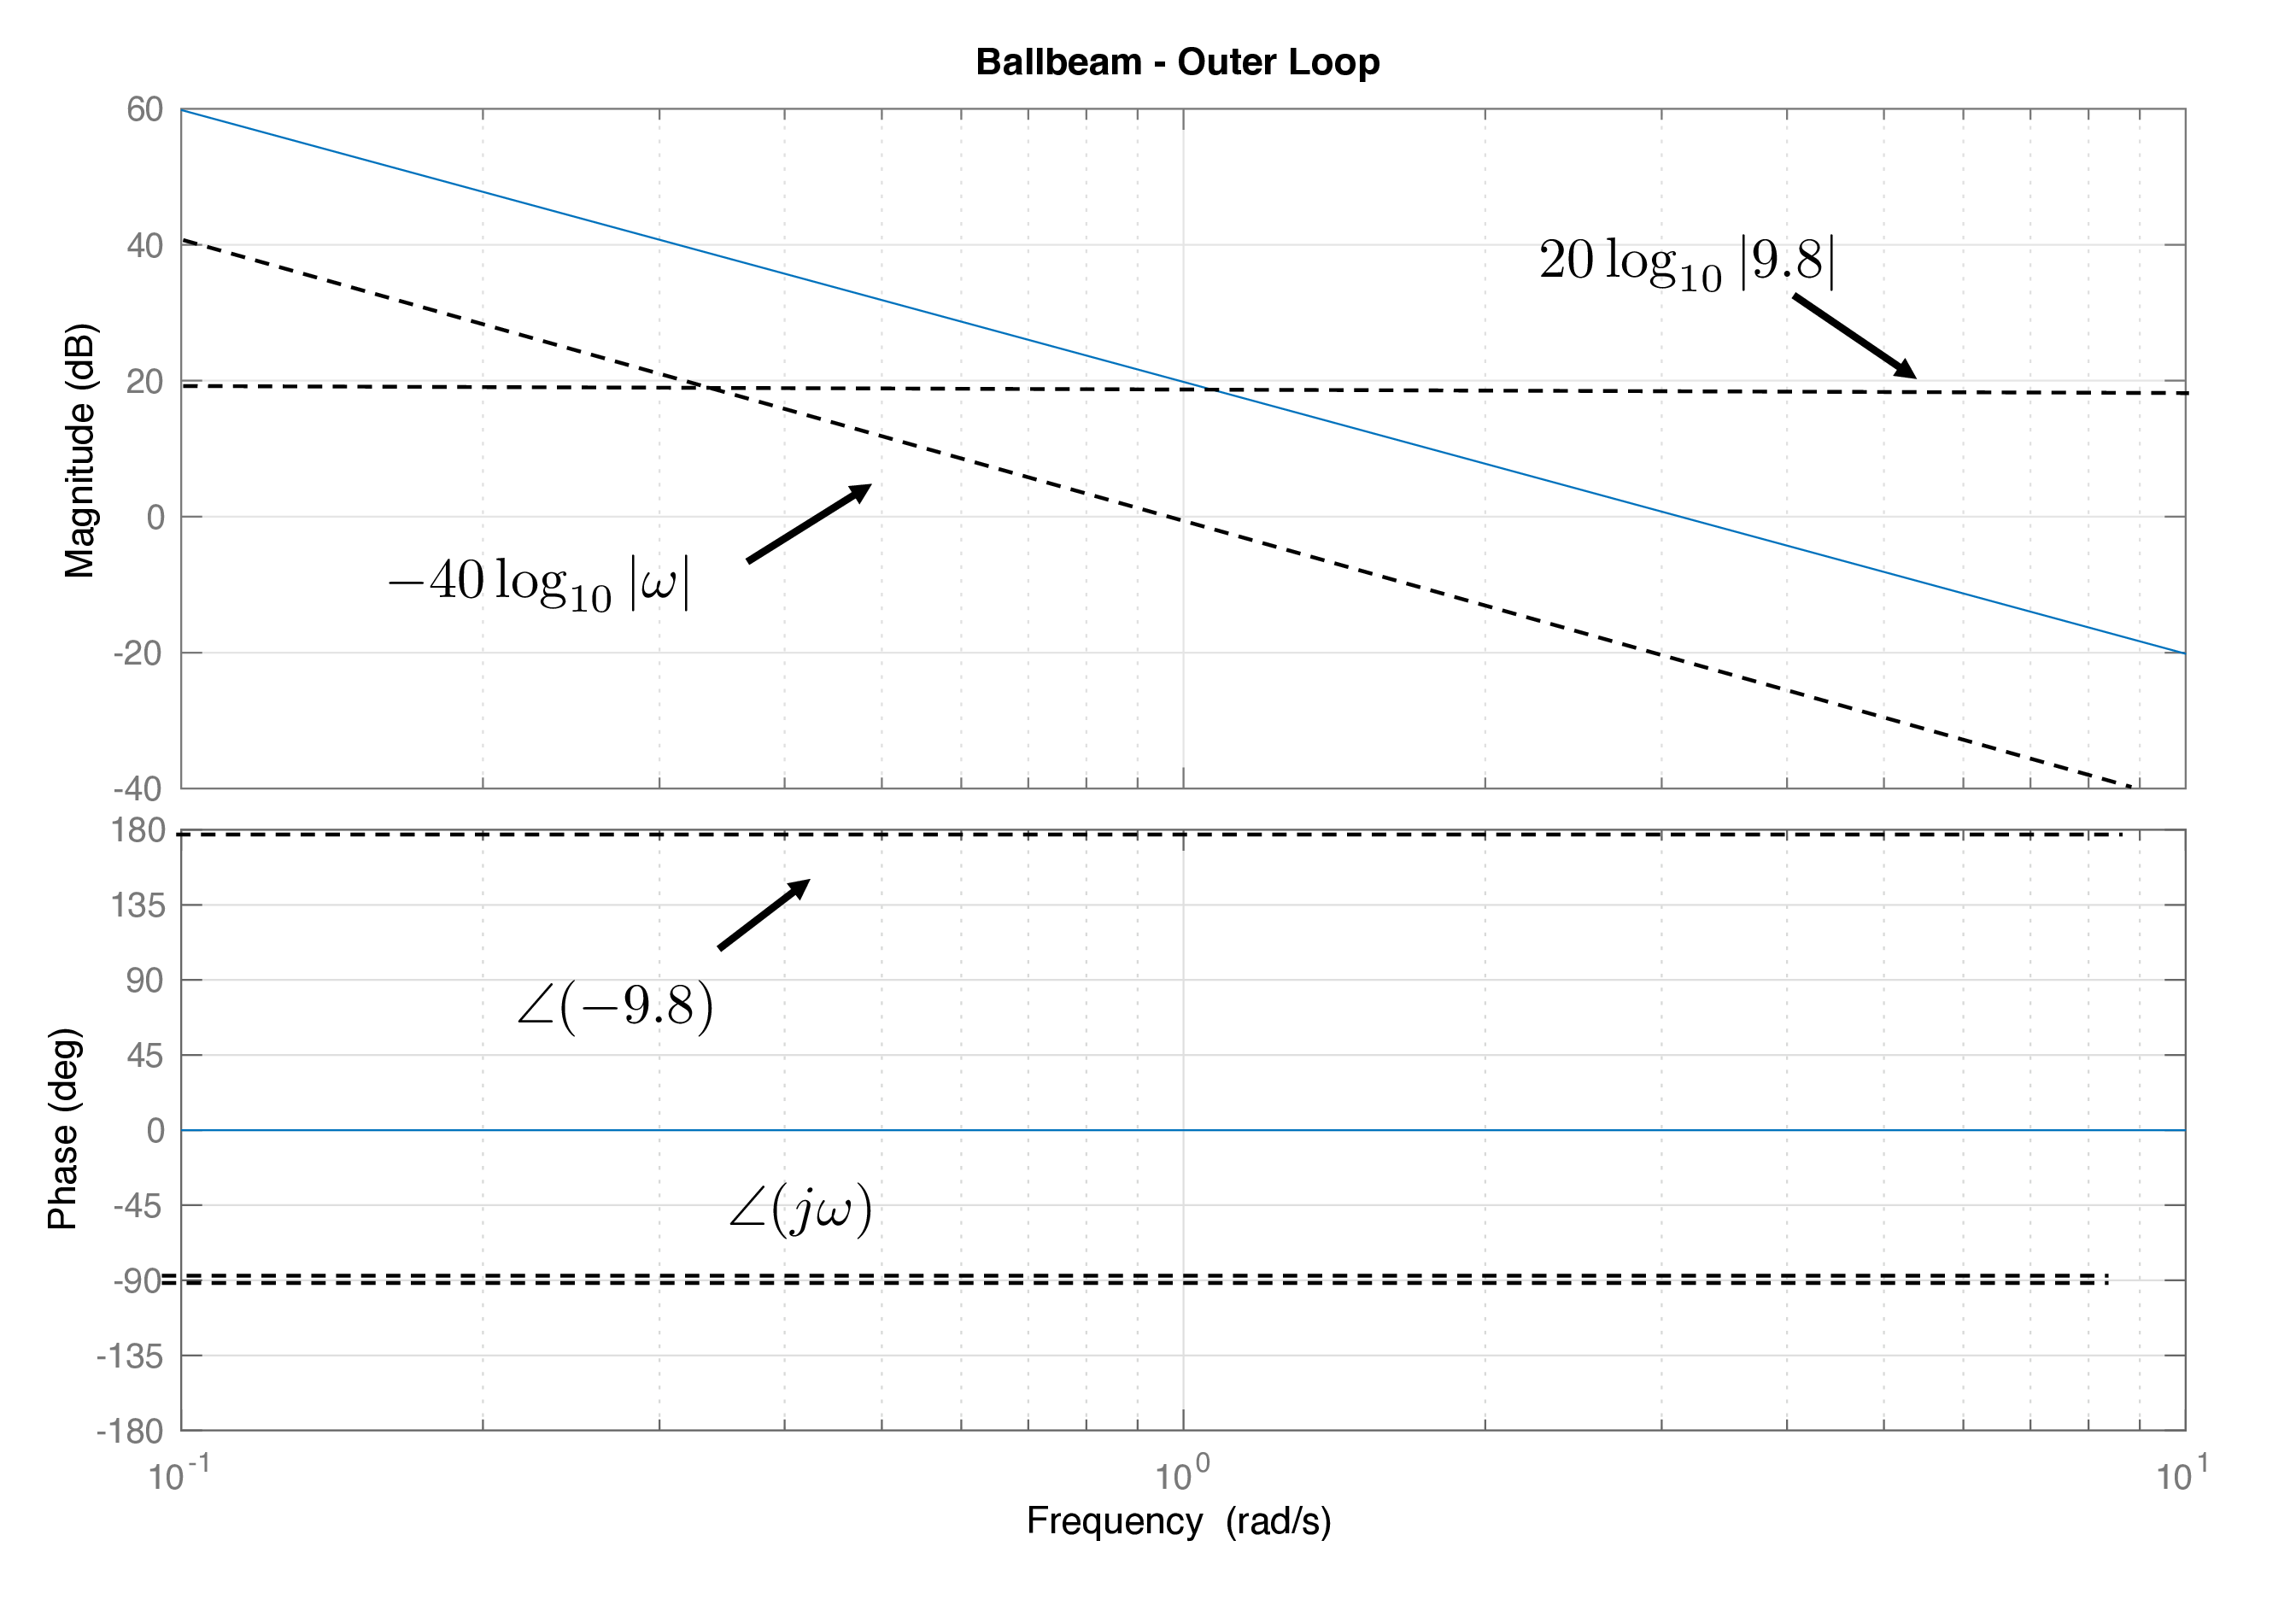
\includegraphics[width=0.9\textwidth]{6_design_studies/figures/hw_ballbeam_bode_out.pdf}
   \caption{Bode plot for the transfer function given in Equation~\eqref{eq:hw_ballbeam_bode_out_tf}.}
   \label{fig:hw_ballbeam_bode_out}
\end{figure}
%The Matlab command to generate the Bode plot is
%\begin{lstlisting}
%>> Pout = tf([-9.8], [1, 0, 0]);
%>> figure(1), clf, bode(Pout), grid on
%\end{lstlisting}
The Python command to generate the Bode plot is
\begin{lstlisting}
	>> import matplotlib.pyplot as plt
	>> import control as cnt
	>> Pout = tf([-9.8], [1, 0, 0]);
	>> plt.figure(1), clf, cnt.bode_plot(Pout), grid on
\end{lstlisting}
